\documentclass{article}

% Language setting
% Replace `english' with e.g. `spanish' to change the document language
\usepackage[english]{babel}

% Set page size and margins
% Replace `letterpaper' with `a4paper' for UK/EU standard size
\usepackage[a4paper,top=2cm,bottom=2cm,left=3cm,right=3cm,marginparwidth=1.75cm]{geometry}

% Useful packages
\usepackage{amsmath}
\usepackage{graphicx}
\usepackage[colorlinks=true, allcolors=blue]{hyperref}
\usepackage{xcolor}
\usepackage{listings}

\colorlet{mygray}{black!30}
\colorlet{mygreen}{green!60!blue}
\colorlet{mymauve}{red!60!blue}

\lstset{
  backgroundcolor=\color{gray!10},  
  basicstyle=\ttfamily,
  columns=fullflexible,
  breakatwhitespace=false,      
  breaklines=true,                
  captionpos=b,                    
  commentstyle=\color{mygreen}, 
  extendedchars=true,              
  frame=single,                   
  keepspaces=true,             
  keywordstyle=\color{blue},      
  language=c++,                 
  numbers=none,                
  numbersep=5pt,                   
  numberstyle=\tiny\color{blue}, 
  rulecolor=\color{mygray},        
  showspaces=false,               
  showtabs=false,                 
  stepnumber=5,                  
  stringstyle=\color{mymauve},    
  tabsize=3,                                     
  title=\lstname 
}


\lstnewenvironment{code}[2][]{%
  \lstset{%
    numbers = left,
    title   = #2,
    #1,
  }%
}{}

\title{Homework 1}
\author{Steinarr Hrafn Höskuldsson}

\newcommand{\mycomment}[1]{}
\usepackage{fancyhdr}
\fancypagestyle{firststyle}
{
   \fancyhf{}
   \fancyhead[L]{Mechatronics 2}
   
   \renewcommand{\headrulewidth}{0pt} % removes horizontal header line
}
\begin{document}

\mycomment{

\begin{figure}[h]
    \centering
    \includegraphics[width=0.75\textwidth]{LAB3/Basic1.png}
    \caption{"Switch test" Breadboard set up}
    \label{fig:Switch_test}
\end{figure}

\lstinputlisting[caption=Defining 'ColorMatch' state, label={lst:colormatch}, language=Python, firstline=44, lastline=52]{LAB3/Basic.py}

} % end of comment

\pagestyle{firststyle}
{\let\newpage\relax\maketitle}

\section{Eclipse}
Getting Eclipse to work was a hassle.

Installed as per the instructions but a few things caused issues beyond what the instructions covered.

The new Arduino IDE version 2 seems to not support the old bootloader of an Arduino Nano, easy solution was to just downgrade to the old version 1.8 .

The AVR plugin on Eclipse seems to have a bug and when creating a project with the AVR Toolchain it doesn't get registered as an AVR project causing Eclipse to refuse to even try uploading, giving error along the lines of: 'AVR project not opened'

I finally found a hack at https://sourceforge.net/p/avr-eclipse/support-requests/38/ which said to paste: 
\verb#<nature>de.innot.avreclipse.core.avrnature</nature># into the \verb".project" file. That fixed that issue and I was on my merry way to every other issue covered in the instructions.

\section{Blink Programs}
Two different blink programs were written, one for the Arduino IDE and another for the Eclipse bare bones.

The Arduino version is just the Arduino Blink example with the delays commented out.

The Eclipse bare bones version was taken from \verb"Baldurs8bitGuide.pdf" .

\section{Speed Comparisons}

The Arduino Nano was connected to a RTB2004 Oscilloscope to measure the time delay between blinks. As can be seen in Figure \ref{hw1:fig:arduino} the Arduino version takes around $3\mu s$ to blink the LED, and not only that but once in a while it takes $9\mu s$. However as can be seen in figure \ref{hw1:fig:eclipse} the bare bones eclipse version takes only $250 ns$.

\begin{figure}[h]
    \centering
    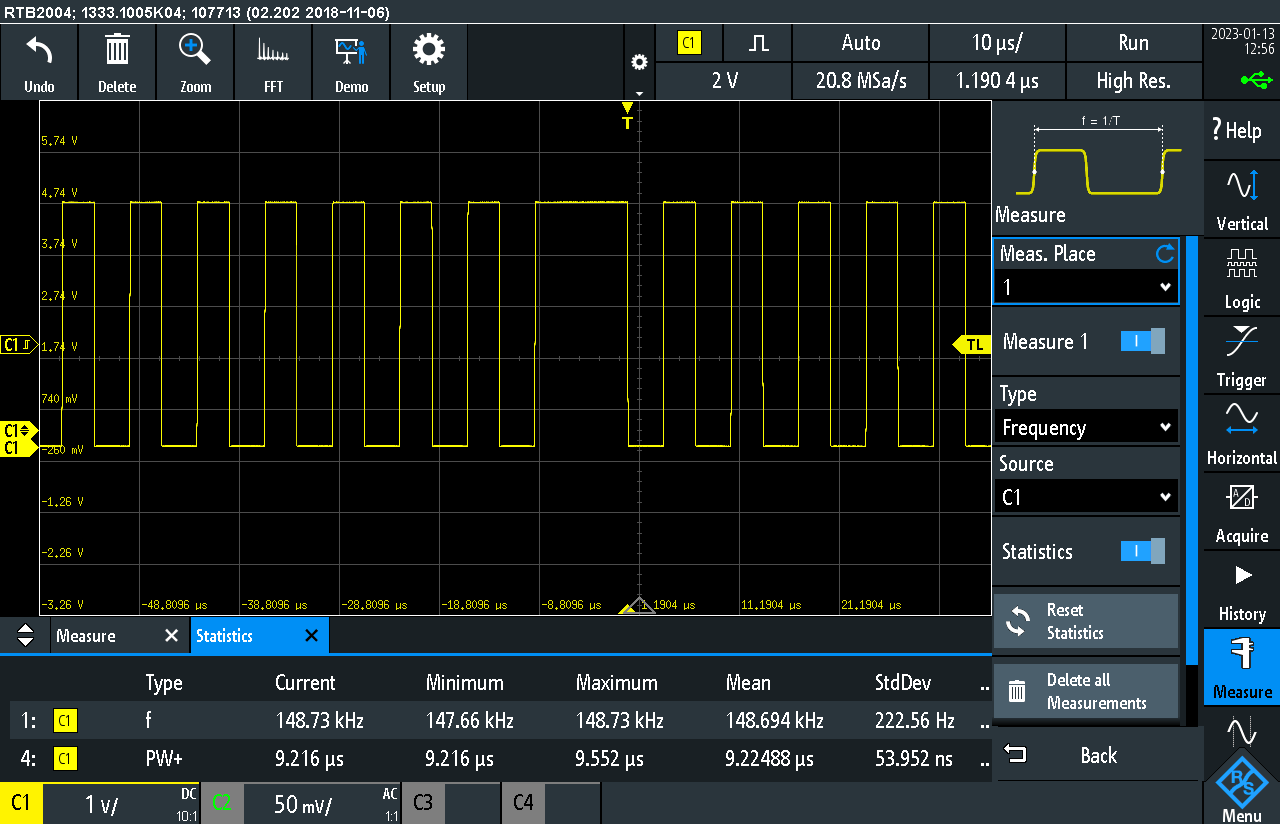
\includegraphics[width=0.75\textwidth]{HW1/ArduinoBlink.PNG}
    \caption{Arduino Blink test, runs at $~150 Khz$ and not consistently}
    \label{hw1:fig:arduino}
\end{figure}


\begin{figure}[h]
    \centering
    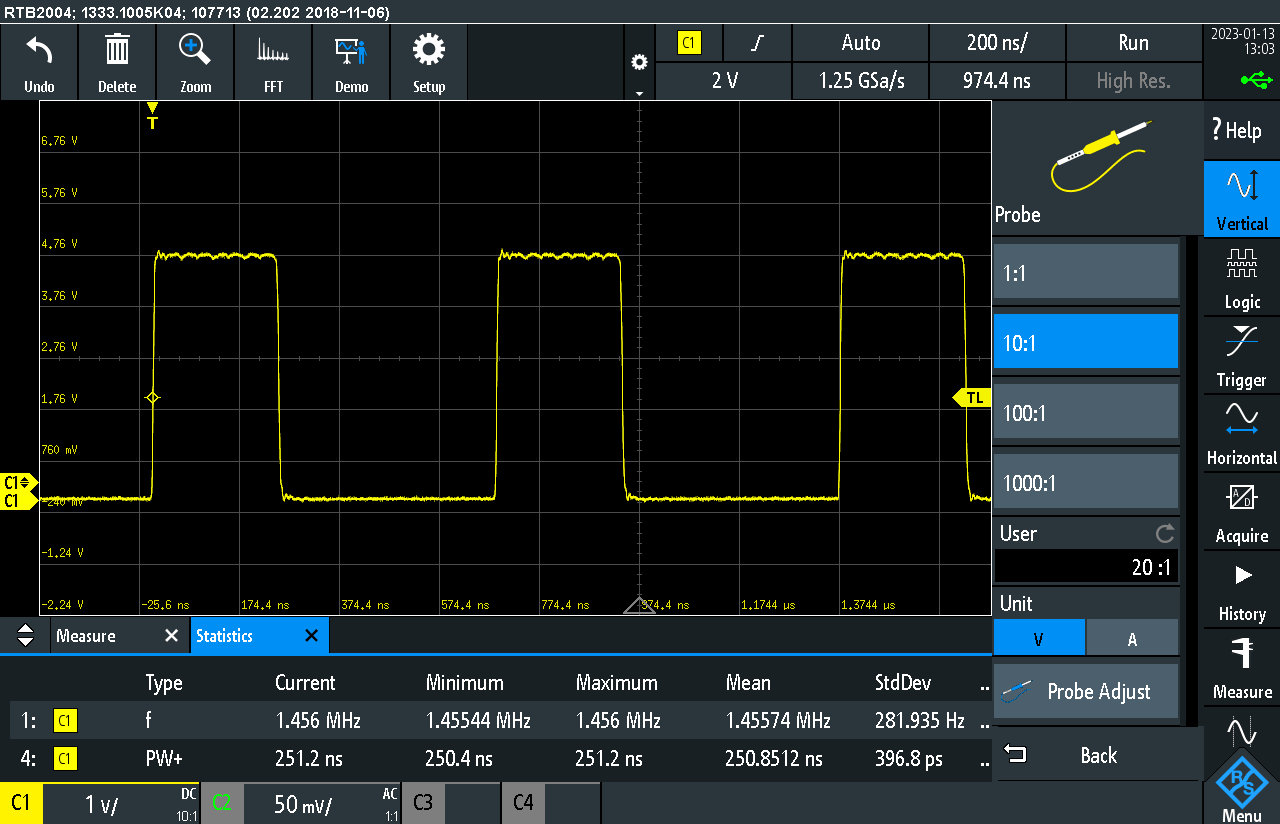
\includegraphics[width=0.75\textwidth]{HW1/EclipseBlink.PNG}
    \caption{Eclipse bare bones Blink test, runs consistently at $1.5 Mhz$}
    \label{hw1:fig:eclipse}
\end{figure}


\section{Assembly Code}

The relevant Assembly instructions for the while loop are:

\begin{verbatim}
    	while (1)
	{
		PORTB = 1<<5 ;
  90:	e5 e2       	ldi	r30, 0x25	; 37
  92:	f0 e0       	ldi	r31, 0x00	; 0
  94:	80 e2       	ldi	r24, 0x20	; 32
  96:	80 83       	st	Z, r24
		PORTB = 0;
  98:	e5 e2       	ldi	r30, 0x25	; 37
  9a:	f0 e0       	ldi	r31, 0x00	; 0
  9c:	10 82       	st	Z, r1
  9e:	f8 cf       	rjmp	.-16     	; 0x90 <main+0x10>

\end{verbatim}
There are some hints that it might be able to run faster, flipping a register bit should be achievable in less than 4 instructions. And indeed it is. By changing the project build properties to heavily optimize the code we get the following assembly instructions.

\begin{verbatim}
    	while (1)
	{
		PORTB = 1<<5 ;
  84:	85 b9       	out	0x05, r24	; 5
		PORTB = 0;
  86:	15 b8       	out	0x05, r1	; 5
  88:	fd cf       	rjmp	.-6      	; 0x84 <main+0x4>
\end{verbatim}

Now each flip of the pin only takes one instruction. A screenshot of the oscilloscope with the optimized code running can be seen in Figure \ref{hw1:fig:optimized}. Interestingly the loop is only 3 instructions,but runs at $4 Mhz$ suggesting that the jump instruction takes 2 clock cycles to execute.  

\begin{figure}[h!]
    \centering
    \includegraphics[width=0.75\textwidth]{HW1/OptimizedBLink.PNG}
    \caption{Optimized Blink test, runs consistently at $4 Mhz$}
    \label{hw1:fig:optimized}
\end{figure}

\newpage
\section{Schematic - Altium}
Altium was installed and a schematic of the setup was created, it can be seen in Figure \ref{hw1:fig:schematic}
\begin{figure}[h!]
    \centering
    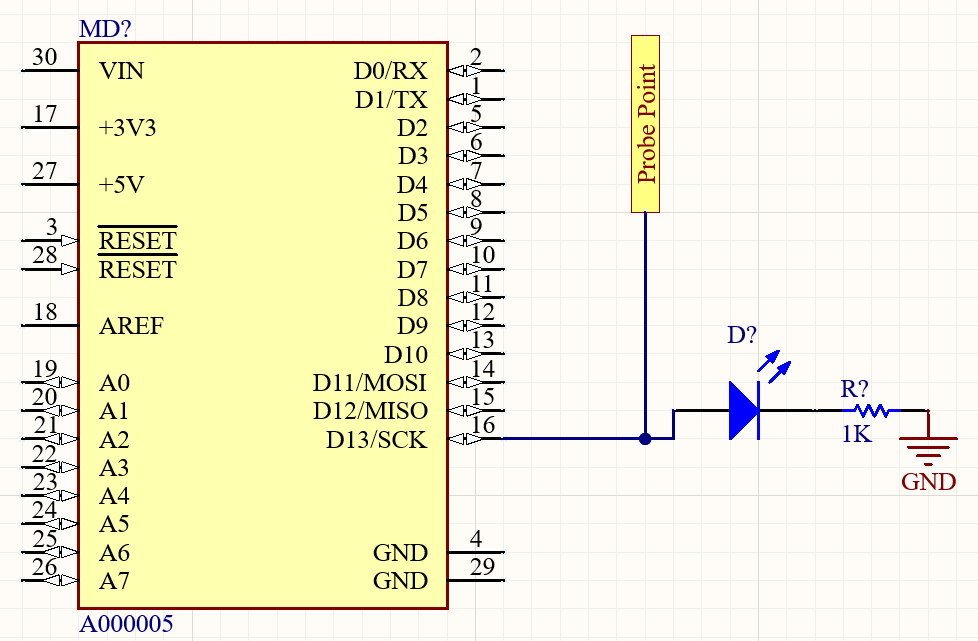
\includegraphics[width=0.75\textwidth]{HW1/schematic.PNG}
    \caption{Schematic of the test setup used.}
    \label{hw1:fig:schematic}
\end{figure}

% JFASDKSDJFLKSDFLKJSDFLKJSDLKJSLDKJFLASKDJFLASKJDFKLASDJFLKSAJDFLKJSADLFKJASDLFK


\newpage
\section{Final Project}
For the final project I propose creating \textbf{AirDrums by Steinarr}, a pair of pants and possibly shoes that contain sensors capable of detecting hand slaps at certain spots as well as foot taps and output what is sensed as drum sounds.

\subsection{Requirements}
The requirements for the device, in order of importance, are
\begin{enumerate}
    \item Detect foot taps on both feet
    \item Detect hand slaps at certain locations, such as thighs.
    \item Create drum sounds from what was sensed.
    \item Allow customization of what sensor makes what sound.
    \item Possibly transmit wirelessly to allow the drummer to dance around if they want.
\end{enumerate}

\subsection{Test plan}
\begin{enumerate}
    \item Test - Sense foot taps and hand slaps with high degree of accuracy ($>99\%$).
    \item Test - Create drum sounds with small enough latency such that it is not noticeable, aim for $5 ms$ or less, $10 ms$ would still be acceptable
    \item  Test - Test a setup sequence to allow user to customize what sensor makes what sound.
    \item Test - Overall feeling when playing the AirDrums by Steinarr
\end{enumerate}

\subsection{Subtasks}
\begin{enumerate}
    \item Choose and test sensors for foot taps and hand slaps
    \item Wire up and Program microcontroller to accurately detect foot taps and hand slaps
    \item Choose and program a method to output sound.
    \item Integrate the results of above steps into one program
    \item Create a setup sequence to allow for customization of the system. 
    \item Choose and program a wireless transceiver to allow the drummer to dance around if they want.
\end{enumerate}

\subsection{Risk factors}
\begin{enumerate}
    \item Sensors not being precise enough, causing missed or erroneous detections.
    \item  
\end{enumerate}

\subsection{Estimated cost}
Estimated Material costs for Arduino Nano, Soundboard, sensors (possibly accelerometers and contact microphones?), wires and other minor electronic components that might be needed:  20.000 ISK

Estimated hours that will be spent on the project: 60

Bringing the total estimated cost to: $60*5.000 + 20.000 = 320.000$ ISK

\newpage
\appendix
\section{Code}\label{appendix:code}

\lstinputlisting[firstline=25, caption=Arduino IDE version of blink program]{HW1/Blink/Blink.ino.ino}

\lstinputlisting[caption=Eclipse bare bones version of blink program]{HW1/main.c}



\end{document}

